% answers.tex —— 2010 年·全国大纲卷Ⅰ·文科 · 参考答案与详细解析片段
% 由 tools/generate_projects.py 依来源总账自 2010/2010_数学真题_全国1文_试题.md + 2010/2010_数学真题_全国1文_解析正文.md + 2010/2010_数学真题_全国1文_答案要点.md 生成，勿手改（改源 MD 后重跑）


\begin{answer}
\gksolhead{1}{}

\textbf{题目}：

$\cos300^\circ=$\mbox{（　　）}

（A）$-\dfrac{\sqrt3}{2}$\quad（B）$-\dfrac12$\quad（C）$\dfrac12$\quad（D）$\dfrac{\sqrt3}{2}$

\Needspace{4\baselineskip}
\textbf{解析}

$\cos300^\circ=\cos(360^\circ-60^\circ)=\dfrac12$，选 C。

\gkanswer{答案：C}

\end{answer}
\begin{answer}
\gksolhead{2}{}

\textbf{题目}：

设全集 $U=\{1,2,3,4,5\}$，集合 $M=\{1,4\}$，$N=\{1,3,5\}$，则 $N\cap\complement_U M=$\mbox{（　　）}

（A）$\{1,3\}$\quad（B）$\{1,5\}$\quad（C）$\{3,5\}$\quad（D）$\{4,5\}$

\Needspace{4\baselineskip}
\textbf{解析}

$\complement_U M=\{2,3,5\}$，故
$N\cap\complement_U M=\{3,5\}$，选 C。

\gkanswer{答案：C}

\end{answer}
\begin{answer}
\gksolhead{3}{}

\textbf{题目}：

\Needspace{5\baselineskip}
若变量 $x,y$ 满足约束条件

\nopagebreak[4]
\[
\begin{cases}
y\leq 1,\\
x+y\geq0,\\
x-y-2\leq0,
\end{cases}
\]

则 $z=x-2y$ 的最大值为\mbox{（　　）}

（A）$4$\quad（B）$3$\quad（C）$2$\quad（D）$1$

\Needspace{4\baselineskip}
\textbf{解析}

可行域的顶点包括 $(-1,1)$、$(3,1)$、$(1,-1)$。分别代入
$z=x-2y$，最大值为 $3$，选 B。

\gkanswer{答案：B}

\end{answer}
\begin{answer}
\gksolhead{4}{}

\textbf{题目}：

已知各项均为正数的等比数列 $\{a_n\}$，$a_1a_2a_3=5$，$a_7a_8a_9=10$，则 $a_4a_5a_6=$\mbox{（　　）}

（A）$5\sqrt2$\quad（B）$7$\quad（C）$6$\quad（D）$4\sqrt2$

\Needspace{4\baselineskip}
\textbf{解析}

\Needspace{5\baselineskip}
设公比为 $q$，则
\nopagebreak[4]
\[
a_7a_8a_9=(a_1a_2a_3)q^{18},
\]
所以 $q^{18}=2$。中间三项的乘积为
$a_4a_5a_6=(a_1a_2a_3)q^9=5\sqrt2$，选 A。

\gkanswer{答案：A}

\end{answer}
\begin{answer}
\gksolhead{5}{}

\textbf{题目}：

$(1-x)^4(1-\sqrt{x})^3$ 的展开式中 $x^2$ 的系数是\mbox{（　　）}

（A）$-6$\quad（B）$-3$\quad（C）$0$\quad（D）$3$

\Needspace{4\baselineskip}
\textbf{解析}

\Needspace{5\baselineskip}
令第二因式取 $1,-3\sqrt{x},3x,-x\sqrt{x}$。$x^2$ 项来自
\nopagebreak[4]
\[
\binom42x^2\cdot1+\binom41(-x)\cdot3x=6-12=-6\text{，}
\]
选 A。

\gkanswer{答案：A}

\end{answer}
\begin{answer}
\gksolhead{6}{}

\textbf{题目}：

直三棱柱 $ABC-A_1B_1C_1$ 中，若 $\angle BAC=90^\circ$，$AB=AC=AA_1$，则异面直线 $BA_1$ 与 $AC_1$ 所成的角等于\mbox{（　　）}

（A）$30^\circ$\quad（B）$45^\circ$\quad（C）$60^\circ$\quad（D）$90^\circ$

\Needspace{4\baselineskip}
\textbf{解析}

\Needspace{5\baselineskip}
取 $A=(0,0,0)$、$B=(1,0,0)$、$C=(0,1,0)$、$A_1=(0,0,1)$，则
\nopagebreak[4]
\[
\overrightarrow{BA_1}=(-1,0,1),\qquad
\overrightarrow{AC_1}=(0,1,1).
\]
两向量的夹角余弦为 $1/2$，故所成角为 $60^\circ$，选 C。

\gkanswer{答案：C}

\end{answer}
\begin{answer}
\gksolhead{7}{}

\textbf{题目}：

已知函数 $f(x)=|\lg x|$。若 $a\neq b$ 且 $f(a)=f(b)$，则 $a+b$ 的取值范围是\mbox{（　　）}

（A）$(1,+\infty)$\quad（B）$[1,+\infty)$\quad（C）$(2,+\infty)$\quad（D）$[2,+\infty)$

\Needspace{4\baselineskip}
\textbf{解析}

函数定义域为正数。若 $|\lg a|=|\lg b|$ 且 $a\neq b$，则
\Needspace{5\baselineskip}
$\lg a=-\lg b$，即 $ab=1$。因此
\nopagebreak[4]
\[
a+b=a+\frac1a\geq2,
\]
等号要求 $a=b=1$，与 $a\neq b$ 矛盾，故 $a+b>2$，选 C。

\gkanswer{答案：C}

\end{answer}
\begin{answer}
\gksolhead{8}{}

\textbf{题目}：

已知 $F_1\text{、}F_2$ 为双曲线 $C:x^2-y^2=1$ 的左、右焦点，点 $P$ 在 $C$ 上，$\angle F_1PF_2=60^\circ$，则 $|PF_1|\cdot|PF_2|=$\mbox{（　　）}

（A）$2$\quad（B）$4$\quad（C）$6$\quad（D）$8$

\Needspace{4\baselineskip}
\textbf{解析}

双曲线焦距为 $2\sqrt2$，设 $PF_1=m$、$PF_2=n$。由双曲线定义
\Needspace{5\baselineskip}
$|m-n|=2$；由余弦定理
\nopagebreak[4]
\[
8=m^2+n^2-mn.
\]
又 $m^2+n^2-2mn=4$，两式相减得 $mn=4$，选 B。

\gkanswer{答案：B}

\end{answer}
\begin{answer}
\gksolhead{9}{}

\textbf{题目}：

正方体 $ABCD-A_1B_1C_1D_1$ 中，$BB_1$ 与平面 $ACD_1$ 所成角的余弦值为\mbox{（　　）}

（A）$\dfrac{\sqrt2}{3}$\quad（B）$\dfrac{\sqrt3}{3}$\quad（C）$\dfrac23$\quad（D）$\dfrac{\sqrt6}{3}$

\Needspace{4\baselineskip}
\textbf{解析}

取正方体边长为 $1$，令 $A=(0,0,0)$、$C=(1,1,0)$、$D_1=(0,1,1)$。
平面 $ACD_1$ 的一个法向量为 $(1,-1,1)$，而
\Needspace{5\baselineskip}
$\overrightarrow{BB_1}=(0,0,1)$。线面角 $\theta$ 满足
\nopagebreak[4]
\[
\sin\theta=\frac1{\sqrt3},qquad \cos\theta=\frac{\sqrt6}{3},
\]
选 D。

\gkanswer{答案：D}

\end{answer}
\begin{answer}
\gksolhead{10}{}

\textbf{题目}：

设 $a=\log_3 2$，$b=\ln2$，$c=5^{-\frac12}$，则\mbox{（　　）}

（A）$a<b<c$\quad（B）$b<c<a$\quad（C）$c<a<b$\quad（D）$c<b<a$

\Needspace{4\baselineskip}
\textbf{解析}

有 $c=1/\sqrt5\approx0.447$、$a=\log_3 2\approx0.631$、
$b=\ln2\approx0.693$，故 $c<a<b$，选 C。

\gkanswer{答案：C}

\end{answer}
\begin{answer}
\gksolhead{11}{}

\textbf{题目}：

已知圆 $O$ 的半径为 $1$，$PA\text{、}PB$ 为该圆的两条切线，$A\text{、}B$ 为两切点，那么 $\overrightarrow{PA}\cdot\overrightarrow{PB}$ 的最小值为\mbox{（　　）}

（A）$-4+\sqrt2$\quad（B）$-3+\sqrt2$\quad（C）$-4+2\sqrt2$\quad（D）$-3+2\sqrt2$

\Needspace{4\baselineskip}
\textbf{解析}

\Needspace{5\baselineskip}
设 $OP=d\geq1$，令 $t=d^2$。由切线长度和夹角关系，
\nopagebreak[4]
\[
\overrightarrow{PA}\cdot\overrightarrow{PB}
=\frac{(t-1)(t-2)}t=t-3+\frac2t.
\]
其最小值在 $t=\sqrt2$ 时取得，为 $-3+2\sqrt2$，选 D。

\gkanswer{答案：D}

\end{answer}
\begin{answer}
\gksolhead{12}{}

\textbf{题目}：

已知在半径为 $2$ 的球面上有 $A\text{、}B\text{、}C\text{、}D$ 四点，若 $AB=CD=2$，则四面体 $ABCD$ 的体积的最大值为\mbox{（　　）}

（A）$\dfrac{2\sqrt3}{3}$\quad（B）$\dfrac{4\sqrt3}{3}$\quad（C）$2\sqrt3$\quad（D）$\dfrac{8\sqrt3}{3}$

\Needspace{4\baselineskip}
\textbf{解析}

设 $U,V$ 为弦 $AB\text{、}CD$ 的中点，$|OU|=|OV|=\sqrt3$，并设半弦向量长度为 $1$。
\Needspace{5\baselineskip}
四面体体积可写为
\nopagebreak[4]
\[
V=\frac23\left|\boldsymbol p\cdot((V-U)\times\boldsymbol q)\right|.
\]
因 $|V-U|\leq2\sqrt3$、$|\boldsymbol p|=|\boldsymbol q|=1$，有
$V\leq4\sqrt3/3$；当 $U\text{、}V$ 对径且方向取到等号时取得，故选 B。

\gkanswer{答案：B}

\end{answer}
\begin{answer}
\gksolhead{13}{}

\textbf{题目}：

不等式 $\dfrac{x-2}{x^2+3x+2}>0$ 的解集是\gkblank{}。

\Needspace{4\baselineskip}
\textbf{解析}

\Needspace{5\baselineskip}
分母为 $(x+1)(x+2)$。作符号分析得
\nopagebreak[4]
\[
x\in(-1,2)\cup(2,+\infty).
\]

\gkanswer{答案：$(-1,2)\cup(2,+\infty)$}

\end{answer}
\begin{answer}
\gksolhead{14}{}

\textbf{题目}：

已知 $\alpha$ 为第二象限的角，$\sin\alpha=\dfrac35$，则 $\tan2\alpha=$\gkblank{}。

\Needspace{4\baselineskip}
\textbf{解析}

\Needspace{5\baselineskip}
第二象限中 $\cos\alpha=-4/5$，故
\nopagebreak[4]
\[
\tan2\alpha=\frac{2\tan\alpha}{1-\tan^2\alpha}
=\frac{2(-3/4)}{1-9/16}=-\frac{24}{7}.
\]

\gkanswer{答案：$-\dfrac{24}{7}$}

\end{answer}
\begin{answer}
\gksolhead{15}{}

\textbf{题目}：

某学校开设 $A$ 类选修课 $3$ 门，$B$ 类选修课 $4$ 门，一位同学从中共选 $3$ 门，若要求两类课程中各至少选一门，则不同的选法共有\gkblank{}种。（用数字作答）

\Needspace{4\baselineskip}
\textbf{解析}

总选法为 $\binom73$，减去只选 $A$ 类的 $\binom33$ 和只选 $B$ 类的
\Needspace{5\baselineskip}
$\binom43$，故
\nopagebreak[4]
\[
\binom73-\binom33-\binom43=35-1-4=30.
\]

\gkanswer{答案：$30$}

\end{answer}
\begin{answer}
\gksolhead{16}{}

\textbf{题目}：

已知 $F$ 是椭圆 $C$ 的一个焦点，$B$ 是短轴的一个端点，线段 $BF$ 的延长线交 $C$ 于点 $D$，且 $\overrightarrow{BF}=2\overrightarrow{FD}$，则 $C$ 的离心率为\gkblank{}。

\Needspace{4\baselineskip}
\textbf{解析}

设椭圆长半轴为 $a$、焦距为 $c$、短半轴为 $b$。取
$F=(c,0)$、$B=(0,b)$，由 $\overrightarrow{BF}=2\overrightarrow{FD}$ 得
\Needspace{5\baselineskip}
$D=(3c/2,-b/2)$。代入椭圆方程并用 $b^2=a^2-c^2$，得
\nopagebreak[4]
\[
\frac{9c^2}{4a^2}+\frac14=1,qquad \frac ca=\frac1{\sqrt3}.
\]

\gkanswer{答案：$\dfrac{\sqrt3}{3}$}

\end{answer}
\begin{answer}
\gksolhead{17}{}

\textbf{题目}：

记等差数列 $\{a_n\}$ 的前 $n$ 项的和为 $S_n$，设 $S_3=12$，且 $2a_1\text{、}a_2\text{、}a_3+1$ 成等比数列，求 $S_n$。

\Needspace{4\baselineskip}
\textbf{解析}

设公差为 $d$。由 $S_3=12$ 得 $a_1+d=4$，即 $a_2=4$。
\Needspace{5\baselineskip}
等比条件给出
\nopagebreak[4]
\[
4^2=2a_1(a_3+1)=2a_1(9-a_1)\text{，}
\]
\Needspace{5\baselineskip}
故 $a_1=1,d=3$ 或 $a_1=8,d=-4$。因此
\nopagebreak[4]
\[
S_n=\frac{n(3n-1)}2\text{，}\quad\text{\text{或}}\quad S_n=2n(5-n).
\]

\gkanswer{答案：$S_n=\dfrac{n(3n-1)}2$ 或 $S_n=2n(5-n)$。}

\end{answer}
\begin{answer}
\gksolhead{18}{}

\textbf{题目}：

已知 $\triangle ABC$ 的内角 $A\text{、}B$ 及其对边 $a\text{、}b$ 满足 $a+b=a\cot A+b\cot B$，求内角 $C$。

\Needspace{4\baselineskip}
\textbf{解析}

\Needspace{5\baselineskip}
由余弦定理，原条件化为
\nopagebreak[4]
\[
4\Delta=(a+b)\bigl[c^2-(a-b)^2\bigr].
\]
结合海伦公式并约去正因子，得
$c^2=a^2+b^2$，所以 $C=90^\circ$。

\gkanswer{答案：$C=90^\circ$。}

\end{answer}
\begin{answer}
\gksolhead{19}{}

\textbf{题目}：

投到某杂志的稿件，先由两位初审专家进行评审。若能通过两位初审专家的评审，则予以录用；若两位初审专家都未予通过，则不予录用；若恰能通过一位初审专家的评审，则再由第三位专家进行复审，若能通过复审专家的评审，则予以录用，否则不予录用。设稿件能通过各初审专家评审的概率均为 $0.5$，复审的稿件能通过评审的概率为 $0.3$。各专家独立评审。

（1） 求投到该杂志的 $1$ 篇稿件被录用的概率；

（2） 求投到该杂志的 $4$ 篇稿件中，至少有 $2$ 篇被录用的概率。

\Needspace{4\baselineskip}
\textbf{解析}

\gksubpart{(1)}

\Needspace{5\baselineskip}
一篇稿件被录用的概率为
\nopagebreak[4]
\[
p=0.5^2+2(0.5)(0.5)(0.3)=0.4.
\]

\gksubpart{(2)}

\Needspace{5\baselineskip}
四篇中至少两篇被录用的概率为
\nopagebreak[4]
\[
\binom42(0.4)^2(0.6)^2+\binom43(0.4)^3(0.6)+(0.4)^4
=\frac{328}{625}.
\]

\gkanswer{答案（1）：$\dfrac25$}

\gkanswer{答案（2）：$\dfrac{328}{625}$}

\end{answer}
\begin{answer}
\gksolhead{20}{}

\textbf{题目}：

如图，四棱锥 $S-ABCD$ 中，$SD\perp$ 底面 $ABCD$，$AB\parallel DC$，$AD\perp DC$，$AB=AD=1$，$DC=SD=2$，$E$ 为棱 $SB$ 上的一点，平面 $EDC\perp$ 平面 $SBC$。
\nopagebreak[4]
\begin{center}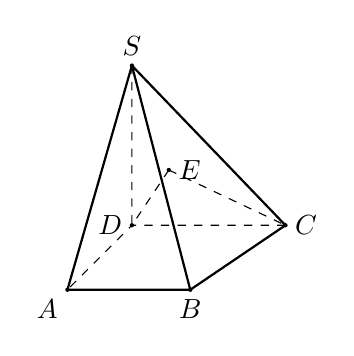
\begin{tikzpicture}[scale=.78,>=stealth]
\coordinate (A) at (0,0); \coordinate (B) at (2.0,0);
\coordinate (C) at (3.55,1.05); \coordinate (D) at (1.05,1.05);
\coordinate (S) at (1.05,3.65); \coordinate (E) at (1.65,1.95);
\draw[thick] (A)--(B)--(C);
\draw[dashed] (C)--(D)--(A) (S)--(D);
\draw[thick] (S)--(A) (S)--(B) (S)--(C);
\draw[dashed] (E)--(D) (E)--(C);
\fill (A) circle (1pt) node[below left] {$A$};
\fill (B) circle (1pt) node[below] {$B$};
\fill (C) circle (1pt) node[right] {$C$};
\fill (D) circle (1pt) node[left] {$D$};
\fill (S) circle (1pt) node[above] {$S$};
\fill (E) circle (1pt) node[right] {$E$};
\end{tikzpicture}
\end{center}
\nopagebreak[4]
（1） 证明：$SE=2EB$；

（2） 求二面角 $A-DE-C$ 的大小。

\Needspace{4\baselineskip}
\textbf{解析}

\gksubpart{(1)}

取 $D=(0,0,0)$、$C=(2,0,0)$、$A=(0,1,0)$、$B=(1,1,0)$、
$S=(0,0,2)$。设 $E=S+t(B-S)$。平面 $SBC$ 的法向量可取 $(1,1,1)$，
平面 $EDC$ 的法向量可取 $(0,-2(1-t),t)$。两平面垂直给出
$3t-2=0$，即 $t=2/3$，所以 $SE=2EB$。

\gksubpart{(2)}

此时 $E=(2/3,2/3,2/3)$。平面 $ADE\text{、}CDE$ 的法向量可分别取
$(1,0,-1)$、$(0,-1,1)$。按题目指定的两侧射线取二面角，法向量内积对应的
余弦为 $-1/2$，故二面角的大小为 $120^\circ$。

\gkanswer{答案（1）：$SE=2EB$}

\gkanswer{答案（2）：二面角 $A-DE-C=120^\circ$。}

\end{answer}
\begin{answer}
\gksolhead{21}{}

\textbf{题目}：

已知函数 $f(x)=3ax^4-2(3a+1)x^2+4x$。

（1） 当 $a=\dfrac16$ 时，求 $f(x)$ 的极值；

（2） 若 $f(x)$ 在 $(-1,1)$ 上是增函数，求 $a$ 的取值范围。

\Needspace{4\baselineskip}
\textbf{解析}

\gksubpart{(1)}

\Needspace{5\baselineskip}
当 $a=1/6$ 时，
\nopagebreak[4]
\[
f'(x)=2(x-1)^2(x+2).
\]
所以 $f$ 在 $(-\infty,-2)$ 上递减，在 $(-2,+\infty)$ 上递增，
极小值为 $f(-2)=-12$，无极大值。

\gksubpart{(2)}

\Needspace{5\baselineskip}
一般地，
\nopagebreak[4]
\[
f'(x)=4(1-x)\bigl[1-3ax(x+1)\bigr].
\]
在 $(-1,1)$ 上恒非负等价于
$-4/3\leq a\leq1/6$。

\gkanswer{答案（1）：极小值为 $-12$（在 $x=-2$ 处取得），无极大值。}

\gkanswer{答案（2）：$-\dfrac43\leq a\leq\dfrac16$。}

\end{answer}
\begin{answer}
\gksolhead{22}{}

\textbf{题目}：

已知抛物线 $C:y^2=4x$ 的焦点为 $F$，过点 $K(-1,0)$ 的直线 $l$ 与 $C$ 相交于 $A\text{、}B$ 两点，点 $A$ 关于 $x$ 轴的对称点为 $D$。

（1） 证明：点 $F$ 在直线 $BD$ 上；

（2） 设 $\overrightarrow{FA}\cdot\overrightarrow{FB}=\dfrac89$，求 $\triangle BDK$ 的内切圆 $M$ 的方程。

\Needspace{4\baselineskip}
\textbf{解析}

\gksubpart{(1)}

设抛物线上参数点为 $(t^2,2t)$。过 $K(-1,0)$ 的弦两端参数为 $t$、$1/t$，
故 $A=(t^2,2t)$、$B=(t^{-2},2/t)$、$D=(t^2,-2t)$。焦点为 $F=(1,0)$。

\gksubpart{(2)}

\Needspace{5\baselineskip}
由题设
\nopagebreak[4]
\[
(t^2-1)(t^{-2}-1)+4=\frac89,
\]
即 $(t+t^{-1})^2=64/9$。计算三角形 $BDK$ 的三边并用加权坐标公式，
\Needspace{5\baselineskip}
其内心为 $(1/9,0)$，内切半径为 $2/3$，所以
\nopagebreak[4]
\[
\left(x-\frac19\right)^2+y^2=\frac49.
\]

\gkanswer{答案（1）：见解析版}

\gkanswer{答案（2）：内切圆 $M$ 的方程为 $\left(x-\dfrac19\right)^2+y^2=\dfrac49$。}

\end{answer}